\documentclass[final,dvipsnames]{beamer}

% ====================
% Packages
% ====================

\usepackage[T1]{fontenc}
\usepackage{tgbonum}
\usepackage[size=a0,orientation=portrait]{beamerposter}
\usetheme{gemini}
\usecolortheme{mit}
\usepackage{graphicx}
\usepackage{subcaption}
\usepackage{booktabs}
\usepackage{tikz}
\usetikzlibrary{trees, matrix, positioning, patterns, shapes, shadows, shapes.arrows, arrows.meta, shapes.multipart, decorations.pathreplacing, calc, tikzmark, shapes.geometric}
\usepackage{pgfplots}
\pgfplotsset{compat=1.14}
\pgfplotsset{every axis/.append style={very thick}}
\usepackage{pgf-pie}
\usepackage[binary-units]{siunitx}
\usepackage{anyfontsize}
\usepackage{amsmath}
\usepackage{mathdots}
\usepackage{mathtools}
\usepackage{bm}
\usepackage[normalem]{ulem}


% ====================
% Lengths
% ====================

% If you have N columns, choose \sepwidth and \colwidth such that
% (N+1)*\sepwidth + N*\colwidth = \paperwidth
\newlength{\sepwidth}
\newlength{\colwidth}
\setlength{\sepwidth}{0.025\paperwidth}
\setlength{\colwidth}{0.3\paperwidth}

\newcommand{\separatorcolumn}{\begin{column}{\sepwidth}\end{column}}

% ====================
% Title
% ====================

\title{\sout{Safe}Tix, The Best-Worst QR-Code Ticketing system}

\author{ Julian Partanen \inst{1} \and Alexander Mattingley-Scott \inst{1}}

\institute[shortinst]{\inst{1} Heidelberg University}

% ====================
% Footer (optional)
% ====================

\footercontent{
	Beginners practical Binary Hacking 2024/25 \hfill
	\href{mailto:me272@uni-heidelberg.de}{tt249@uni-heidelberg.de}}
% (can be left out to remove footer)

% ====================
% Logo (optional)
% ====================

% use this to include logos on the left and/or right side of the header:
%\logoright{\includegraphics[height=6cm]{}}
%\logoleft{\includegraphics[height=6cm]{}}

% ====================
% Body
% ====================

\begin{document}

\begin{frame}[t, fragile]
\begin{columns}[t]
\separatorcolumn

\begin{column}{\colwidth}

    \begin{block}{About the original SafeTix}
        \begin{itemize}
            \item Ticketmaster is an American ticket sales and distribution company \cite{ticketmaster_wikipedia}
            \item For all kinds of events like concerts, sport events, theater and more \cite{ticketmaster_wikipedia}
            \item Some partners: Taylor Swift, NFL, NHL, NBA, WWE, AEW, theater productions like Harry Potter and the Cursed Child and many more \cite{ticketmaster_wikipedia}
            \item SafeTix: Rotating ticketing system by ticketmaster, initially introduced in 2019 \cite{introducing_safetix} \cite{ticketmaster_safetix_faq} \cite{nba_safetix_faq}
            \begin{figure}[h]
                \begin{center}
                    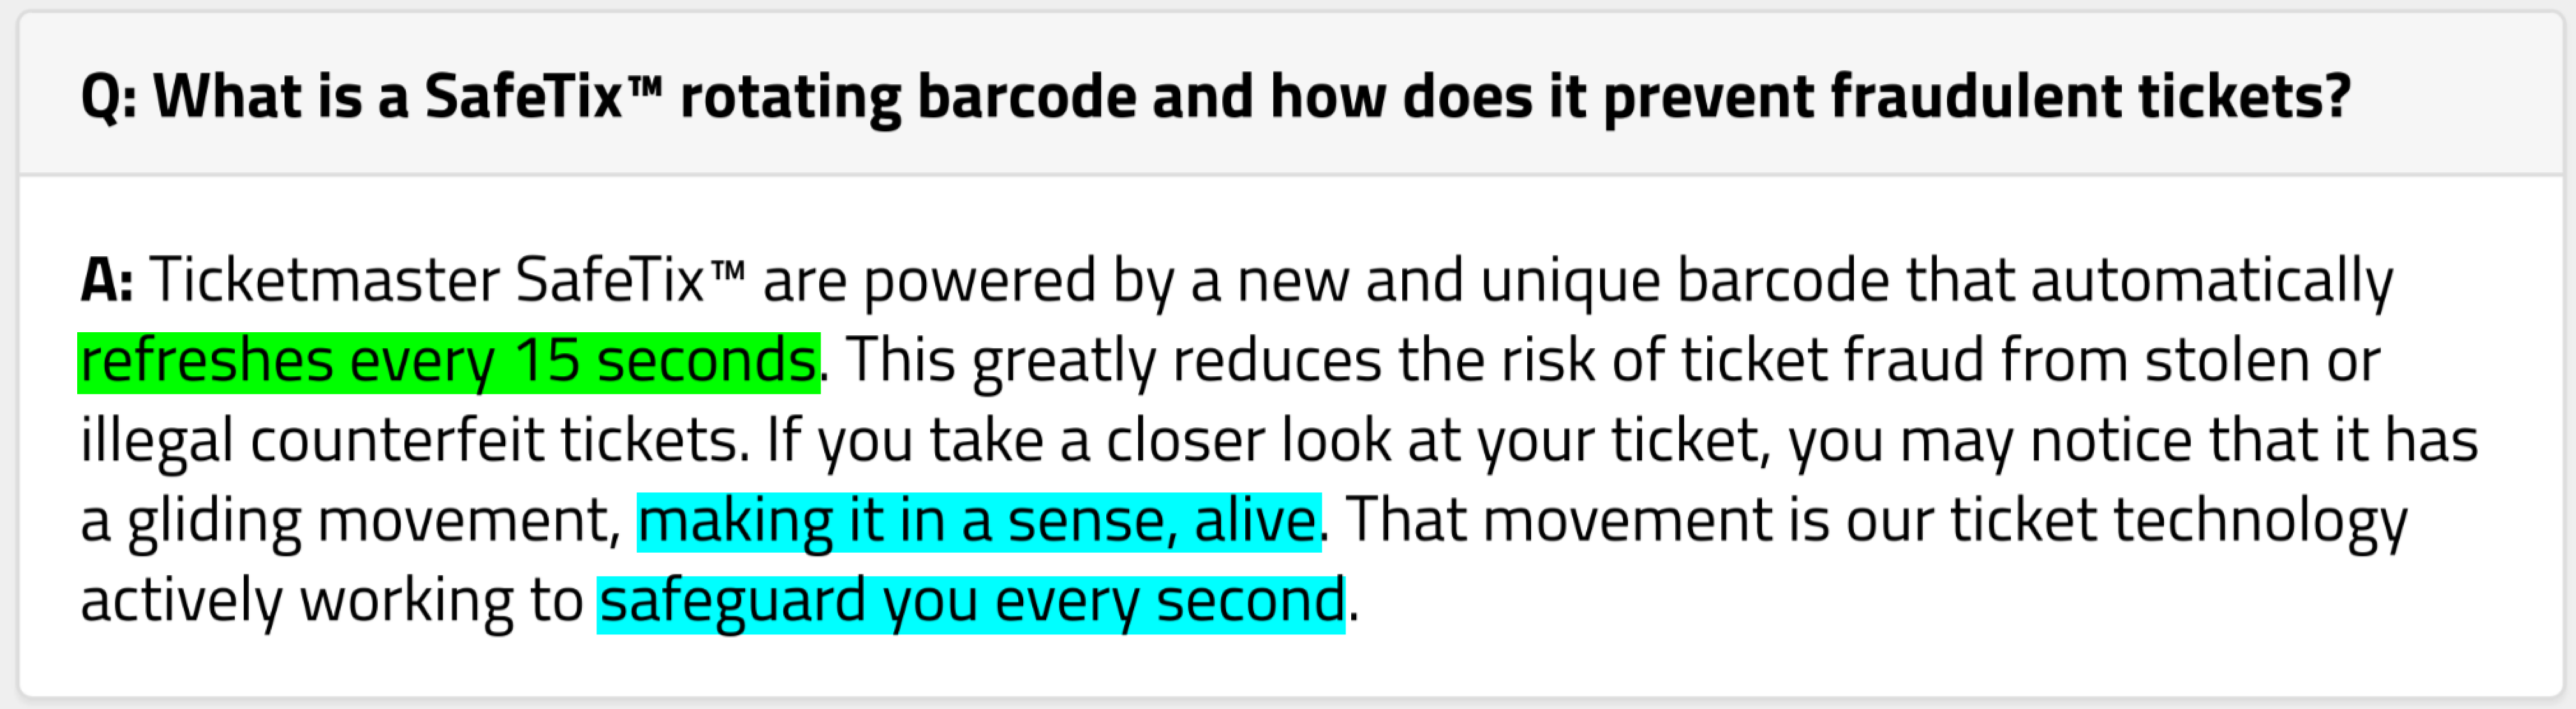
\includegraphics[width=\textwidth]{figures/SafeTix_Quote_1.png}
                \end{center}
                \begin{center}
                    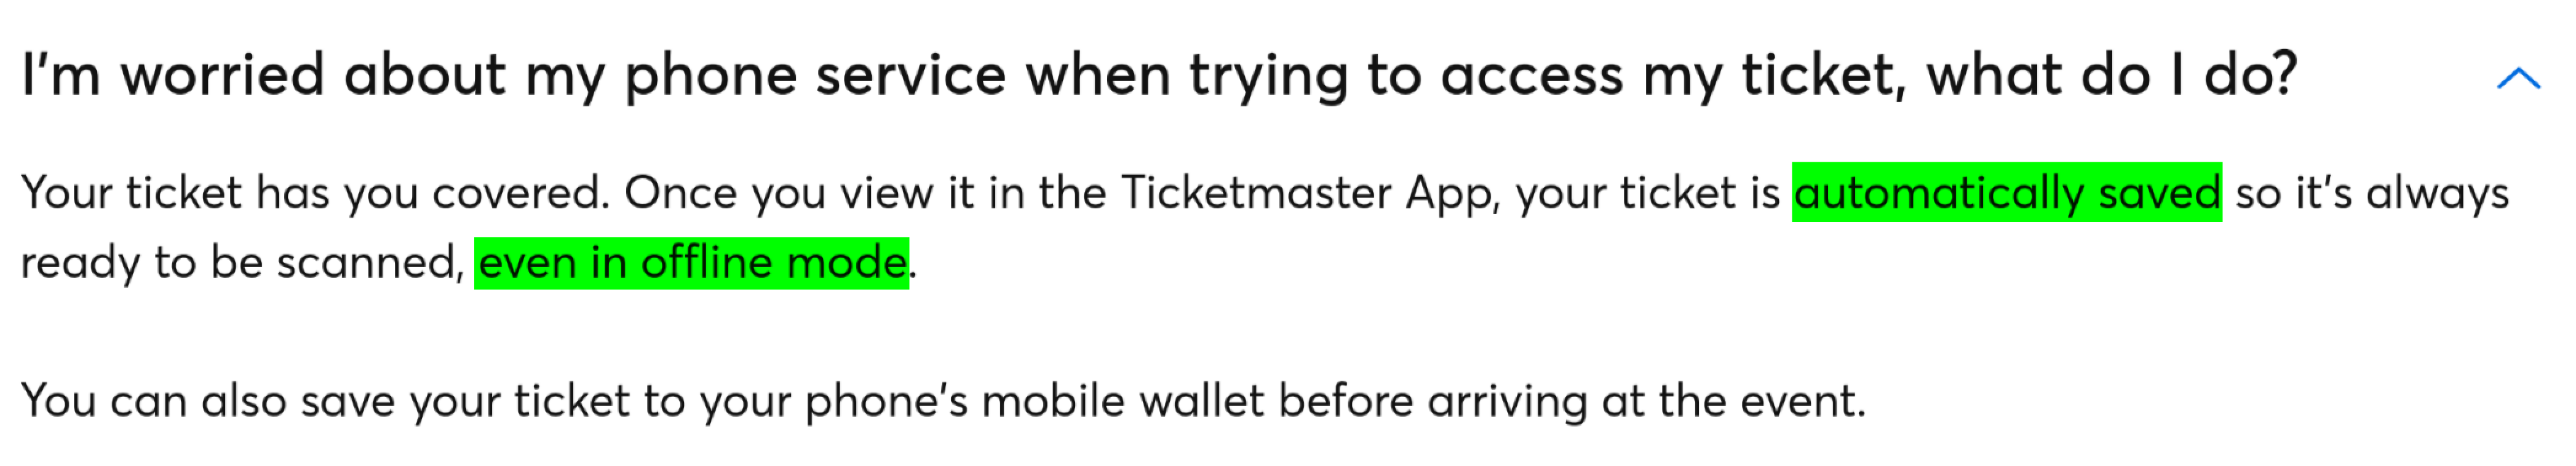
\includegraphics[width=\textwidth]{figures/SafeTix_Quote_2.png}
                \end{center}
                \caption{Two quotes from ticketmaster's and NBA's FAQ pages about SafeTix \cite{ticketmaster_safetix_faq} \cite{nba_safetix_faq}}
                \label{fig:safetix_quotes}
            \end{figure}
            \item Barcode changes every 15 seconds, making transfers through screenshots or printouts impossible \cite{nba_safetix_faq}
            \item However ticket still works offline (once the ticket has been downloaded once) \cite{ticketmaster_safetix_faq}
        \end{itemize}

        \begin{figure}[h]
            \centering
            \begin{subfigure}{.5\textwidth}
                \centering
                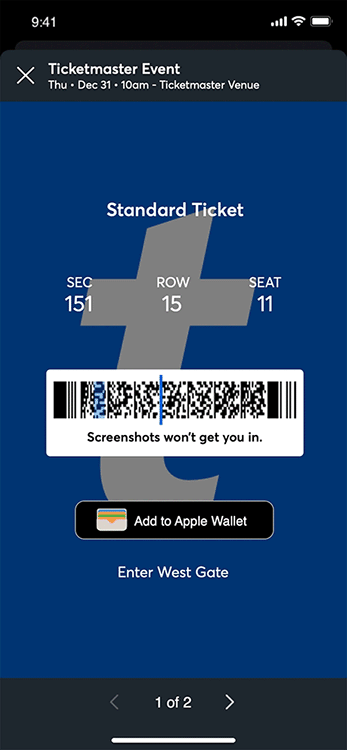
\includegraphics[width=1\linewidth]{figures/SafeTix_App_Barcode.png}
                \caption{A screenshot from ticketmaster's app showing SafeTix in action \cite{ticketmaster_mobile_ticketing}}
                \label{fig:app_barcode}
            \end{subfigure}%
            \begin{subfigure}{.5\textwidth}
                \centering
                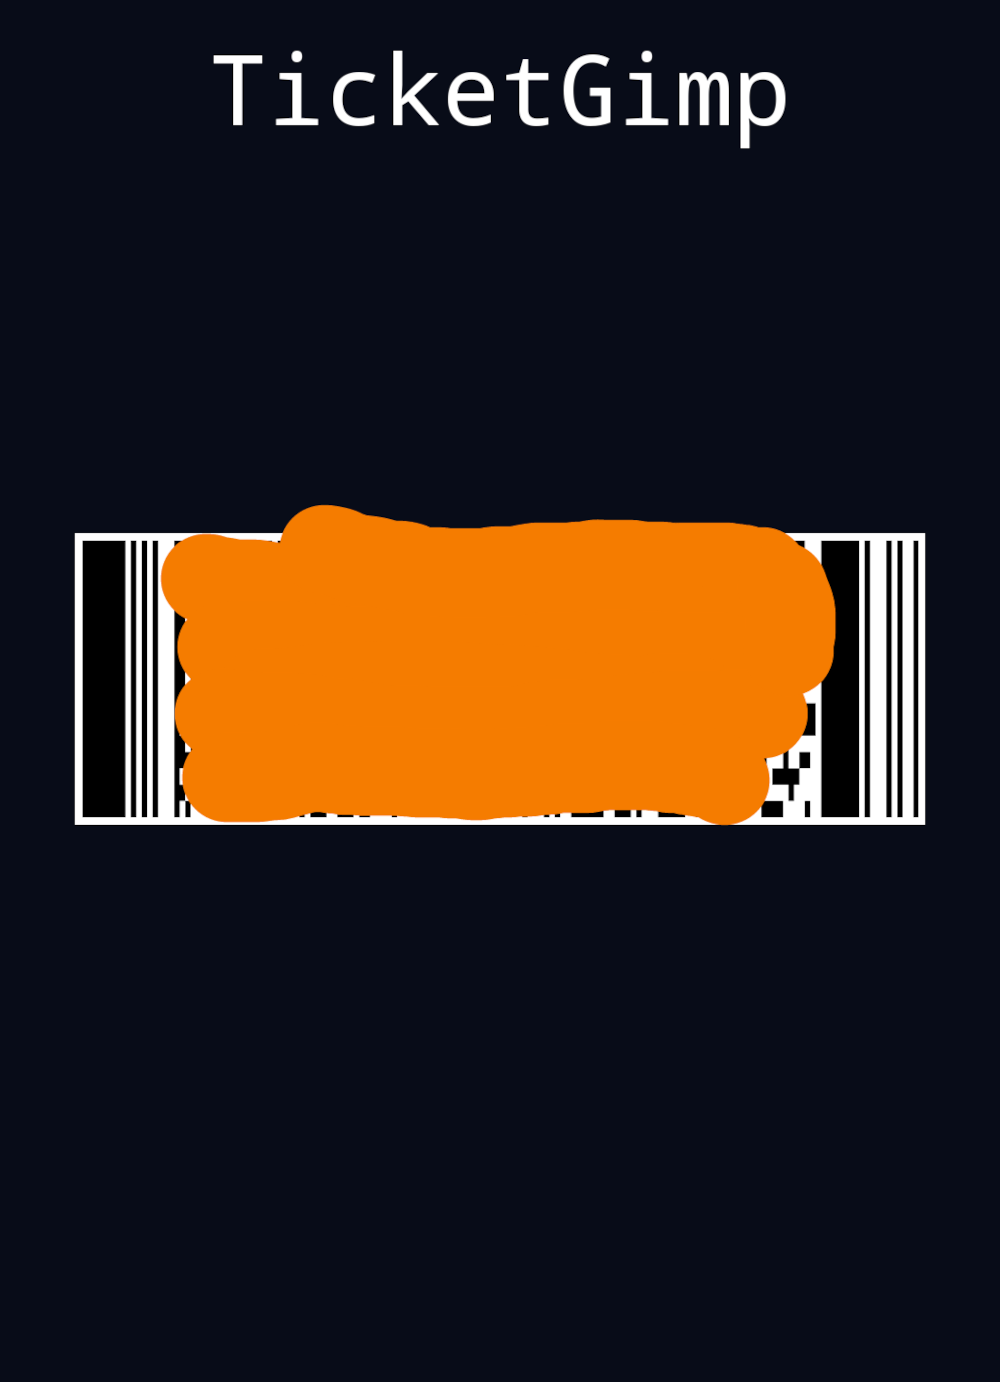
\includegraphics[width=1\linewidth]{figures/Conduition_custom_ticket_app.png}
                \caption{The Expo app Conduition called TicketGimp Conduition wrote to store and render the extracted tickets \cite{reverse_engineering_ticketmaster}}
                \label{fig:conduition_custom_app}
            \end{subfigure}
            \caption{Official ticketmaster App vs. custom app for extracted tickets}
        \end{figure}
    \end{block}

    \begin{block}{How SafeTix got cracked}
        \begin{quotation}
            “Screenshots won’t get you in”, but Chrome DevTools will.
        \end{quotation}
        \begin{itemize}
            \item The Rust/Crypto developer Conduition reverse engineered SafeTix
            \item They managed to extract the ticket of ticketmaster's app into their own app and used that to enter the venue
            \item They described the process in a blog post \cite{reverse_engineering_ticketmaster}
            \item The barcode consists of a static bearer token and two rotating numbers \cite{reverse_engineering_ticketmaster}
            \item Rotating numbers: Standard TOTP (except only valid for 15 seconds instead of 30)
            \item TOTP secrets can be extracted from WebApp using either debug tools to analyse network traffic or by just reading the terminal output
        \end{itemize}
    \end{block}
\end{column}

\separatorcolumn

\begin{column}{\colwidth}

    \begin{block}{Introducing: \sout{Safe}Tix, the binary hacking challenge}

		\begin{itemize}
			\item For our project, we decided to recreate a QR code scanner that mimics the behavior of SafeTix. 
			SafeTix, a digital ticketing system used by TicketMaster, claims to enhance security through dynamically rotating QR codes. 
			However, we found an article that takes a closer look at its implementation and reveals significant vulnerabilities that undermine its effectiveness.

			The Safetix system generates time-based one-time passwords (TOTPs) using an event-specific key and a customer-specific key, with a 15-second time step. 
			While this is meant to prevent duplication, the raw token containing this data is easily extractable from the web application’s source code. 
			In fact, TicketMaster logs the token directly to the browser console, making it trivial for attackers to capture and reuse it.
			This flaw enables unauthorized duplication, resale, or offline storage of tickets—effectively bypassing TicketMaster’s restrictions. 
			Additionally, there is uncertainty about the lifetime of raw tokens, raising concerns about the extent to which SafeTix can prevent ticket fraud.
			\begin{figure}[h] % "h" means place here
				\centering
				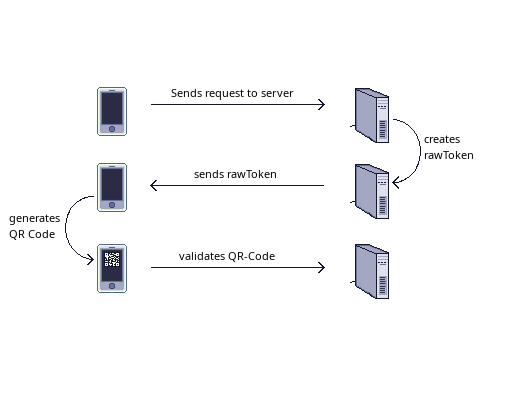
\includegraphics[width=0.9\textwidth]{figures/Image_1.png} % Adjust width as needed
				\caption{The Program for dummies I guess ?.}
				\label{fig:sample}
			\end{figure}
			By recreating SafeTix, we aimed to make it a notch safer (not logging the ticket to the console) but keep a vulnerability that can be reverse engineered. 
			\item 
		\end{itemize}

	\end{block}

\end{column}

\separatorcolumn

\begin{column}{\colwidth}

	\begin{block}{References}
		%\nocite{*}
		\footnotesize{\bibliographystyle{ieeetr}\bibliography{poster.bib}}
	\end{block}

\end{column}

\separatorcolumn
\end{columns}
\end{frame}

\end{document}
